\documentclass{imc-inf}

\title{Multimodal Large Language Models (LLMs) in Medical Imaging}
\subtitle{Great Call for Open Source}
\thesistype{Review Report} % or Bachelor Expos\'e
\author{David Fodor}
% \supervisor{Dr. Supervisor Musterfrau}
\copyrightyear{2021}
\submissiondate{19.04.2021}
\keywords {Data Analytics, Machine Learning, Useability} % add keywords here 



% \usepackage{xyz}
% ... add your own packages here!
\usepackage{listings}
\usepackage{subcaption}
\usepackage{csquotes} 

\begin{document}
\frontmatter\maketitle{}


\begin{declarations}\end{declarations}



\begin{abstract}
	Abstract paragraphs should be unindented. Abstract text must fit on a single page. Try to present the essence of your work here. 
	
	According to Wikipedia\footnote{https://en.wikipedia.org/}, An abstract is a brief summary of a research article, thesis, review, conference proceeding, or any in-depth analysis of a particular subject and is often used to help the reader quickly ascertain the paper's purpose \cite{988366}. When used, an abstract always appears at the beginning of a manuscript or typescript, acting as the point-of-entry for any given academic paper or patent application. Abstracting and indexing services for various academic disciplines are aimed at compiling a body of literature for that particular subject.
	
	It is usually not a good practice to include references and footnotes in an abstract. Abstracts must be independent of other works, concise and complete in itself. 
	
	It is also possible to write structured abstracts. These are abstracts with distinct, labeled sections (e.g., Introduction, Methods, Results, Discussion), which makes it easier for the reader to navigate easily through the content. 
	
\end{abstract}


\begin{acknowledgements}
This is an \textbf{optional} page. Use your choice of paragraph style for text on this page. Usually, this space is for thanking your supporters and getting emotional about how grateful you are to everyone.  
\end{acknowledgements}

\addtoToC{Table of Contents}%
\tableofcontents%
\clearpage


\addtoToC{List of Tables}%
\listoftables
\clearpage


\addtoToC{List of Figures}%
\listoffigures
\clearpage


%   MAIN MATTER  %%%%%%%%%%%%%%%%%%%%%%%%%%%%%%%%%%%%%%%%%%%%%%%%%%%%%%%%%%%%%%
\mainmatter%

\chapter{Introduction}\label{chap:introduction}

The topic of choice chosen for this report was \textbf{Multimodal Large Language Models (LLMs) in Medical Imaging}.
The reason for this choice is quite simple actually, in the last few months I personally took interest in the topic of locally runnable models.
My goal for this report is to provide a brief overview of the topic as set out by task description, with extra focus on the open source aspect of the topic.
Exploring it deeper through a practical project is not part of the task, but makes the report more interesting and engaging.

\section{LLMs and the Move to Multimodality}

The world of health sciences and medical imaging is not new to the use of machine learning and artificial intelligence.
In fact, several artificial intelligence methods have been applied to a variety of tasks, including image classification, segmentation, detection, reconstruction, registration, and computer-aided diagnosis, but all of these traditional approaches are simple, unimodal models that are highly specialized and trained to do specific tasks, making it difficult to apply them to different scenarios.\cite{rajendran2025foundation}
While these are all very helpful tools for medical professionals, they can merely accelerate and assist decision-making due to their inflexible nature and lack of contextual understanding.
It offers better insight for medical professionals to interpret, but lacks the actual "intelligence" to give a complex diagnosis or an actual proposal of a treatment plan.

TODO: Figure showcasing classical AI methods in medical imaging.

LLMs generally work by processing and generating text based on the input they receive and the the patterns they have learned during training on massive amounts of data.
This training on diverse datasets allows them to understand a wide range of subjects and contexts, combined with their ability to generate coherent and contextually relevant human-like text that makes it a prime candidate for chatbot applications, virtual assistants, and other natural language processing tasks.
This interpretation of the unimodal LLMs has the ability to reason and understand complex relationships between concepts, which is exacly what the classical AI methods in medical imaging lack.
Only issue is that these unimodal LLMs are limited to processing and generating text.

This is where Multimodal language models (MLLMs) come into play, as they are designed to process and depending on the model even generate multiple types of data, such as text, images, audio, and video.
For the introduction of MLLMs I will rely on the work of Nam et al., who described the concept of MLLMs compared to LLMs as the following:

\begin{displayquote}[Nam et al. \textit{Multimodal Large Language Models in Medical Imaging: Current State and Future Directions}\cite{nam2025multimodal}]
    MLLMs extend these capabilities [of LLMs] by incorporating advanced computer vision modules and multimodal learning techniques. 
	The defining feature is their ability to integrate and align information across modalities, often mapping them into a shared representational space.
	This synergy allows for a more comprehensive understanding than unimodal approaches permit.
	Consequently, MLLMs can tackle complex crossmodal tasks such as radiology report generation (RRG) from images and visual question answering (VQA) that incorporates both imaging and clinical context.
\end{displayquote}

\begin{figure}[htbp]
    \centering
    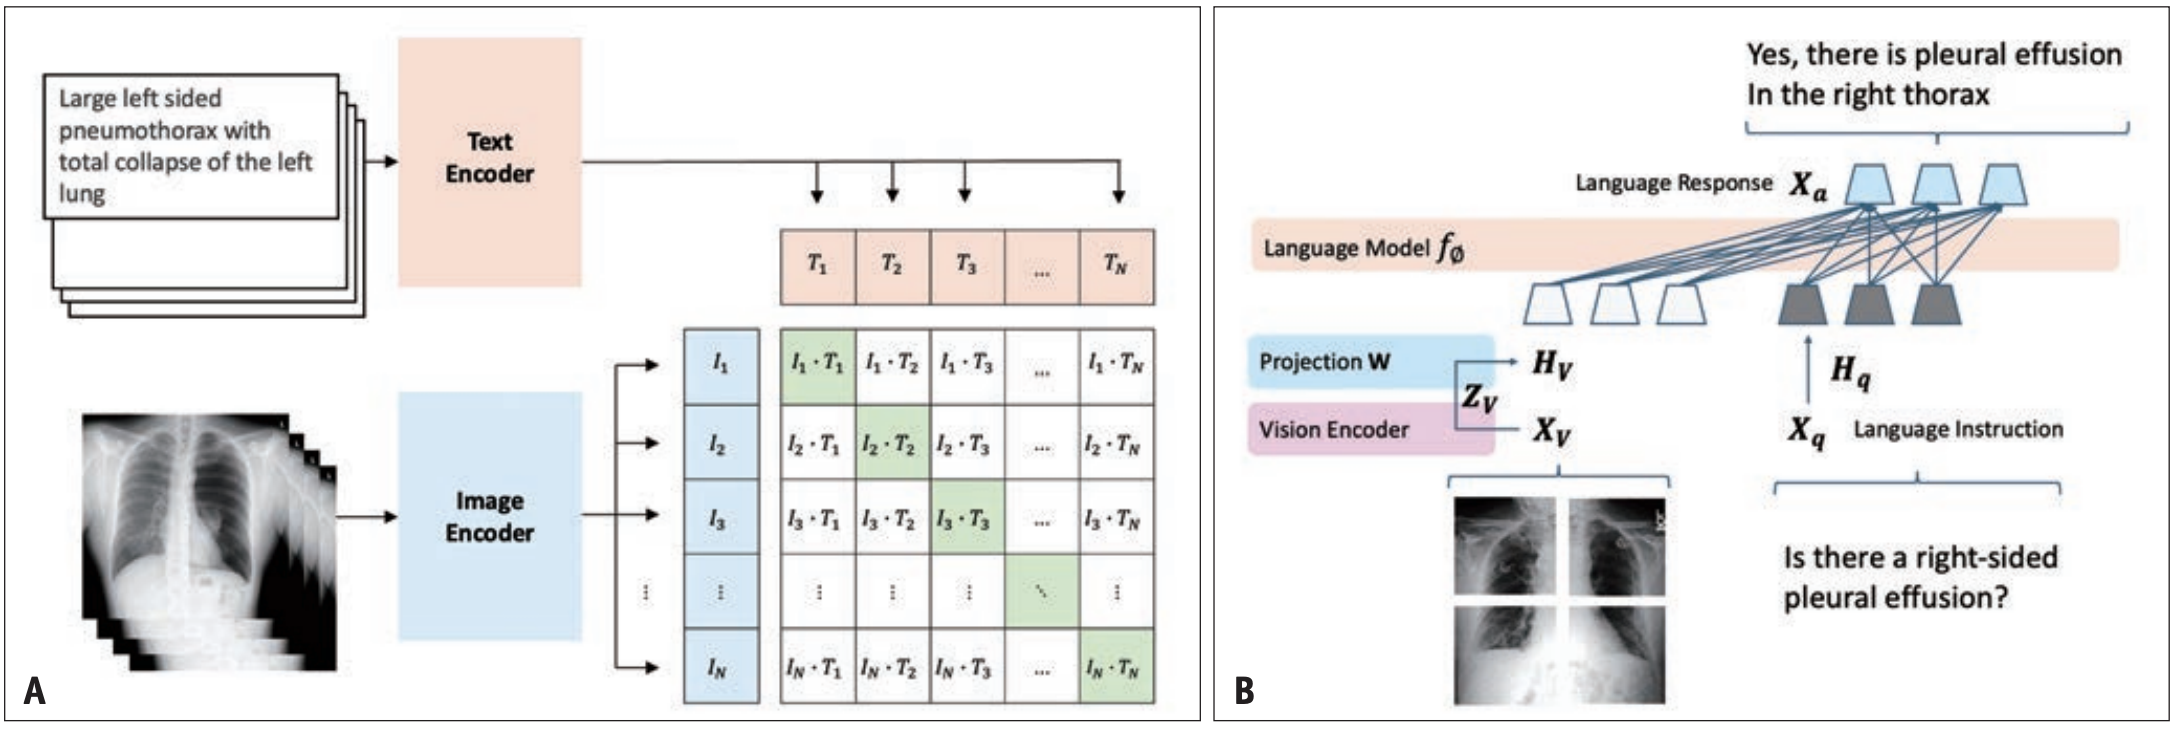
\includegraphics[width=0.8\textwidth]{src/multimodal.png}
    \caption{Visual representation of the training step of an MLLM (A) and the inference step of an MLLM (B). As adapted by Nam et al.\cite{nam2025multimodal}.}
    \label{fig:myimage}
\end{figure}

Multimodal LLMs have the potential to revolutionize the field of medical imaging by further empowering medical professionals with greater insights or even completely automating certain aspects of the diagnostic process.
Instead of relying on multiple specialized unimodal models used for specific data types, MLLMs make use of multimodal encoders and connectors to transform non-textual data into a format that can be processed and understood by the underlying larger scale LLM.\cite{nam2025multimodal}
In the above example of a CT scan, the raw image would first be encoded to make it easier to work with, and then the connector would transform the encoded image into a format that can be processed by the LLM, which can then generate a radiology report based on the image and any additional clinical context provided.

Following this brief overview of the technology, in the following chapters we will discuss the state of the art in terms of models and approaches, as well as performance and benchmarks, followed by a discussion on the challenges and limitations of MLLMs in medical imaging, and finally an exploration of open source models and their relevance in practice, with a practical example showcasing how easy it is to run a multimodal LLM locally on your own machine.

\chapter{Research}\label{chap:research}

Never stop experimenting.

\section{State of the Art - Models and Approaches}

Never stop experimenting.

\section{State of the Art - Performance and Benchmarks}

\cite{hou2025one} - RSNA Case of the day / comparison of common models

\cite{nakaura2025performance} - performance of MLLMs on chest X-ray datasets

\cite{sheng2026multimodal} - NEJM multimodal LLM performance benchmarks

\cite{llmstats2026} - general multimodal LLM performance benchmarks


Examples of papers proposing new benchmarks for MLLMs in medical imaging:

\cite{liu2025medq} - MedQ - benchmark proposed to evaluate the performance of MLLMs in medical imaging tasks, shows that there is a long way to go before can be used as automated
\cite{peng2026omnibrainbench} - Omnibrainbench - benchmark proposed to evaluate the performance of MLLMs in brain imaging tasks, shows a lot better performance for humans and highlights that open source models were lagging behind at the time of writing

Never stop experimenting.

\chapter{Challenges and Limitations}

Never stop experimenting.

\cite{alsaad2024multimodal} - challenges and limitations of MLLMs in medical imaging

\cite{li2026gmai} - brings up the issue of not having enough medical data - tries solving the solution through GMAI-VL dataset specialized training
\cite{moglia2026minigpt} - create a specialized MLLM based of pancreas imaging, shows that specialized models can outperform generalist models in specific tasks - demonstrates that compact MLLMs can rival specialized vision networks in pancreas imaging, offering an intuitive, language-driven tool for AI-assisted radiology

\chapter{Open Source}

\cite{chen-etal-2024-towards-injecting} - example of specializing open source MLLM models for medical imaging tasks

Never stop experimenting.

\section{Open VS Closed Source}

Never stop experimenting.

Relevance of Local Models in Practice - privacy, security, data protection, and compliance with regulations such as HIPAA and GDPR.

\section{Excurse: Running a Multimodal LLM Locally}

Never stop experimenting.

nejm-02-05-26
  Expected:      Pulmonary mucormycosis
  No options:    Invasive pulmonary aspergillosis
  With options:  Pulmonary mucormycosis

nejm-03-19-26
  Expected:      Walled-off pancreatic necrosis
  No options:    Infected pancreatic necrosis (likely with gas formation/abscess)
  With options:  Walled-off pancreatic necrosis

nejm-06-04-26
  Expected:      Osteosarcoma
  No options:    Osteosarcoma
  With options:  Osteosarcoma

  
\chapter{Conclusions and Future Outlook}

Never stop experimenting.

\cite{alsaad2024multimodal} - future outlook

\chapter{Self-Reflection}

Never stop experimenting.

\backmatter%
	\addtoToC{Bibliography}
	\bibliographystyle{IEEEtranS}
 \typeout{}
	\bibliography{references}
	

\begin{appendices} % optional
\chapter{Example Appendix 1}

Appendices should be used for supplemental information that does not form part of the main research. Remember that figures and tables in appendices should not be listed in the List of Figures or List of Tables. 

\chapter{Example Appendix 2}

Appendices should be used for supplemental information that does not form part of the main research. Remember that figures and tables in appendices should not be listed in the List of Figures or List of Tables. 
	
\end{appendices}
\end{document}
